\chapter{SEEDS using Depth Information}
\label{chapter:seeds-depth}

This chapter covers the main topic of this thesis and presents extensions of \textbf{SEEDS} \cite{VanDenBerghBoixRoigCapitaniVanGool:2012} utilizing depth information. In particular, we aim to preserve the framework given by \textbf{SEEDS}, which can best be described as the combination of block and pixel updates, while improving the generated superpixel segmentation. As described in sections \ref{section:seeds-depth-3d-mean-pixel-updates} and \ref{section:seeds-depth-3d-normal-mean-pixel-updates}, integrating depth information into pixel updates can be done similar to \textbf{SLIC3D} and \textbf{DASP} \cite{WeikersdorferGossowBeetz:2012}. However, in our opinion, block updates are responsible for the excellent runtime of \textbf{SEEDS} and therefore we discuss several approaches to improve block updates using depth as well.

% Integrating depth information into \textbf{SEEDS} \cite{VanDenBerghBoixRoigCapitaniVanGool:2012} was the main focus of this thesis. In particular, we wanted to preserve the framework of \textbf{SEEDS}, which can be described as the combination of block and pixel updates, while enhancing the generated superpixel segmentation using depth.
%\begin{algorithm}[b!]
%	\begin{algo}{SEEDS (framework)}{\label{algo:seeds-depth-framework}\qinput{color image $I$, initial block size $w^{(l)} \times h^{(l)}$, histogram size $Q$}\qoutput{superpixel segmentation $S$}}
%		initialization\\
%		\qfor $l = L - 1$ \qto 1\\
%			\qforeach block $B_i^{(l)}$ at level $l$\\
%				perform block update for block $B_i^{(l)}$\qrof\qrof\\
%		\qfor $n = 1$ \qto $N$\\
%			perform pixel update for pixel $x_n$
%	\end{algo}
%	\caption[The basic framework implemented by \textbf{SEEDS} \cite{VanDenBerghBoixRoigCapitaniVanGool:2012}.]{At its heart, \textbf{SEEDS} uses block updates and pixel updates to refine an initial superpixel segmentation.}
%	\label{fig:seeds-depth-framework}
%\end{algorithm}

% As we see in section \ref{section:seeds-depth-3d-mean-pixel-updates} and \ref{section:seeds-depth-3d-normal-mean-pixel-updates}, integrating depth information into pixel updates works similar to \textbf{SLIC3D} and \textbf{DASP} \cite{WeikersdorferGossowBeetz:2012}. Therefore, we focussed on integrating depth information into block updates, because in our opinion, block updates are the main reason for the excellent runtime of \textbf{SEEDS}.

\section{3D Pixel Updates}
\label{section:seeds-depth-3d-mean-pixel-updates}

Similar to \textbf{SLIC3D}, it is possible to integrate 3D point coordinates into mean pixel updates by changing the distance in equation \eqref{eq:superpixel-segmentation-seeds-distance} to
\begin{align}
	\label{eq:seeds-deth-ed-mean-pixels-distance}
	d(x_n, S_j) = \|I(x_n) - I(S_j)\|_2 + \beta\|P(x_n) - P(S_j)\|_2
\end{align}
where $\beta$ can be interpreted as parameter controlling compactness of superpixels within three dimensional space. Using mean pixel updates with the above distance function is referred to as \textbf{SEEDS3D}.
%A suitable normalization is given by
%\begin{align}
%	P =& \left(\max_{x_i} \{P_1(x_i)\} - \min_{x_i} \{P_1(x_i)\}\right)^2 + \left(\max_{x_i} \{P_2(x_i)\} - \min_{x_i} \{P_2(x_i)\}\right)^2\\
%	& + \left(\max_{x_i} \{P_3(x_i)\} - \min_{x_i} \{P_3(x_i)\}\right)^2.
%\end{align}
%Then, algorithm \ref{algo:seeds-depth-3d-mean-pixel-updates} describes the resulting procedure.
%\begin{algorithm}[b!]
%	\begin{algo}{SEEDS (3D mean pixel updates)}{\label{algo:seeds-depth-3d-mean-pixel-updates}\qinput{color image $I$, initial block size $w^{(1)} \times h^{(1)}$, histogram size $Q$}\qoutput{superpixel segmentation $S$}}
%		initialization\\
%		block updates\\
%		\qcom{Initialize superpixel centers}\\
%		\qfor $k = 1$ \qto $K$\\
%			calculate $I(S_k)$ and $P(S_k)$\qrof\\
%		\qfor $n = 1$ \qto $N$\\
%			let $S_j$ be the superpixel $x_n$ belongs to\\
%			\qif a neighboring pixel belongs to a different superpixel $S_k$\\
%				\qthen \qif $d(x_n, S_k) < d(x_n, S_j)$\\
%					\qthen $S_k$ \qlet $S_k \cup \{x_n\}$, $S_j$ \qlet $S_j - \{x_n\}$\qfi\qfi\qrof\\
%		\qreturn $S$
%	\end{algo}
%	\caption{\textbf{SEEDS} extended to use 3D point coordinates for pixel updates.}
%	\label{fig:seeds-depth-3d-mean-pixel-updates}
%\end{algorithm}

\subsection{Discussion}

Although simple, experiments in chapter \ref{chapter:evaluation} show that usage of 3D point coordinates for pixel updates slightly increases performance. This observation can be explained by considering that pixel updates have the greatest influence on the final superpixel segmentation. Therefore, depending on the parameter $\beta$, the above pixel updates are capable of adapting the initial superpixel segmentation to the underlying three dimensional structure. This includes boundaries within the depth image as well as more difficult boundaries between objects in highly cluttered scenes where the above distance prevents superpixels to cover multiple objects and enforces compactness on the object's surface. In contrast to \textbf{VCCS} \cite{PaponAbramovSchoelerWoergoetter:2013}, however, when using a small $\beta$, superpixels may still cover multiple objects even if these objects are not connected in the sense of a voxelized point cloud. Furthermore, the block updates remain unaffected such that the complexity remains unchanged. Figure \ref{fig:seeds-depth-3d-mean-pixels-comparison} shows the running examples oversegmented using \textbf{SEEDS3D}.
\begin{figure}[t]
	\centering
	\subfigure{
		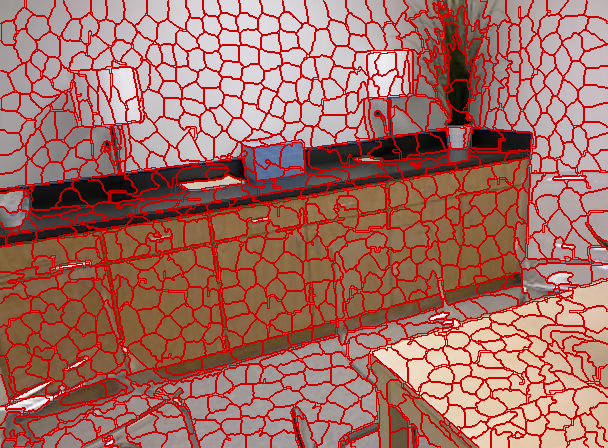
\includegraphics[scale=\scalefivenyu]{pictures/nyu-1-seeds3d}
	}
	\subfigure{
		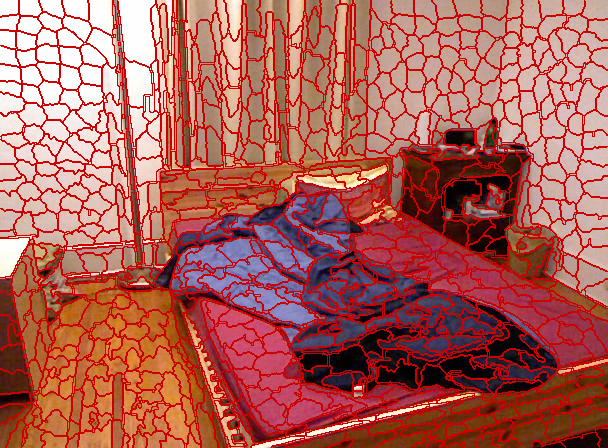
\includegraphics[scale=\scalefivenyu]{pictures/nyu-2-seeds3d}
	}
	\subfigure{
		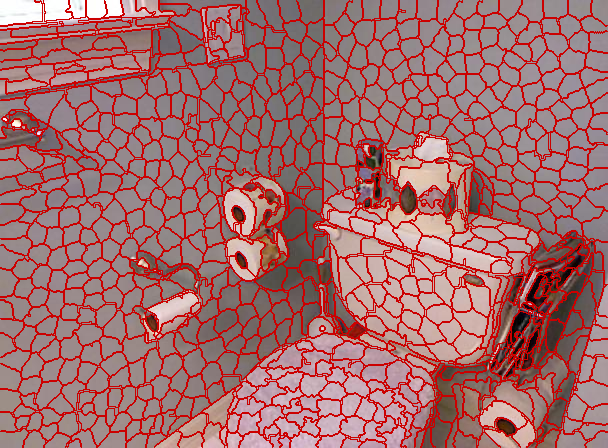
\includegraphics[scale=\scalefivenyu]{pictures/nyu-3-seeds3d}
	}
	\subfigure{
		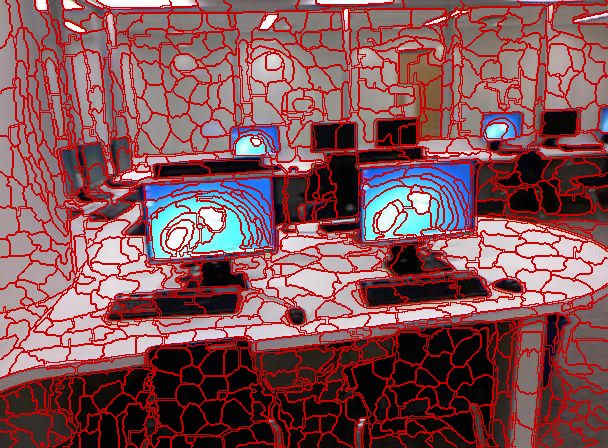
\includegraphics[scale=\scalefivenyu]{pictures/nyu-4-seeds3d}
	}
	\subfigure{
		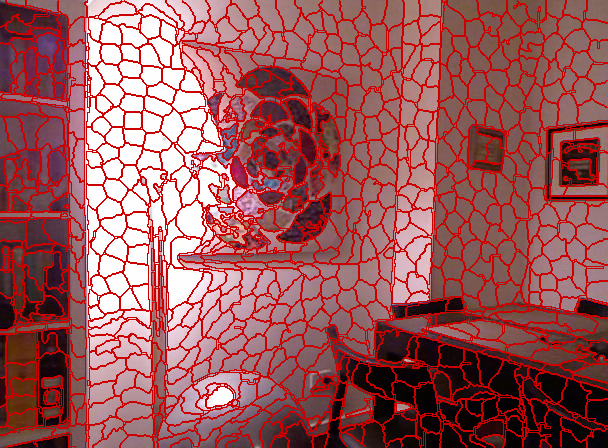
\includegraphics[scale=\scalefivenyu]{pictures/nyu-5-seeds3d}
	}
	\caption[The running examples oversegmented by an extension of \textbf{SEEDS} \cite{VanDenBerghBoixRoigCapitaniVanGool:2012} using 3D point coordinates for pixel updates.]{The running examples oversegmented into exactly $840$ superpixels using \textbf{SEEDS3D}. Further examples are available in section \ref{subsection:evaluation-comparison-qualitative} and appendix \ref{chapter:appendix-evaluation}.}
	\label{fig:seeds-depth-3d-mean-pixels-comparison}
\end{figure}

\section{3D Pixel Updates using Normal Information}
\label{section:seeds-depth-3d-normal-mean-pixel-updates}

Similar to \textbf{DASP}, normal information can be integrated into pixel updates by adapting equation \eqref{eq:seeds-deth-ed-mean-pixels-distance} to
\begin{align}
	\label{eq:seeds-depth-3d-normal-mean-pixels-distance}
	d(x_n, S_j) = \|I(x_n) - I(S_j)\|_2 + \beta\|P(x_n) - P(S_j)\|_2 + \gamma  \arccos \left(N(x_n)^T N(S_j) \right)
\end{align}
where $\beta$ is a compactness parameter and $\gamma$ controls the influence of normal information. Instead of computing the arc-cosine of the dot product $N(x_n)^T N(S_j)$, a distance similar to the one utilized by \textbf{DASP} can be used. This variant of \textbf{SEEDS3D} is in the following referred to as \textbf{SEEDS3Dn}.

The problem of estimating the normal $N(x_n)$ for the point $P(x_n)$ based on a set of points $P(x_{n_1}), \ldots, P(x_{n_k})$ within its local neighborhood is discussed in detail in \cite{Rusu:2009} and several implementations are available as part of the Point Cloud Library \cite{RusuCousins:2011}. For example, using the covariance matric $C$ of the points $P(x_n), P(x_{n_1}), \ldots, P(x_{n_k})$, the normal $N(x_n)$ can be estimated by computing the eigenvalues and eigenvectors of $C$. This corresponds to a first order plane fit. As we can base normal estimation on an ordered point cloud constructed from the depth image $D$, normals can be computed efficiently using integral images, see \cite{HolzerRusuDixonGedikliNavab:2012}. In contrast, \textbf{VCCS} uses least squares plane fits to compute normals within an unordered point cloud and \textbf{DASP} estimates normals purely based on the depth gradient $\nabla D$.

% Computing normals, given a point cloud, can be done using different approaches. In \cite{KlasingAlthoffWollherrBuss:2009} two methods are distinguished: optimization based methods and averaging methods. In general, the problem can be stated as follows: Given a set of points $P(x_1), \ldots, P(x_N)$, we want to estimate a normal $N(x_n)$ for each point using a local neighborhood around the point. For details we refer to \cite{KlasingAlthoffWollherrBuss:2009}. Normals for \textbf{VCCS} are estimated using a least squares plane fit (see the documentation of the Point Cloud Library \cite{Rusu:2009}), while the normals for \textbf{DASP} are based on the depth gradient computed using finite differences. %As discussed in \cite{Rusu:2009}, the normals are not consistently oriented such that they will need to be oriented towards the viewpoint.

\subsection{Discussion}

While normal estimation can be done quite efficiently and results in eligible normal estimates, these are still quite noisy and lack accuracy especially in highly cluttered scenes and at object borders, see figure \ref{fig:seeds-depth-3d-normal-mean-pixels-normal-computation}. Additionally, normals estimated for regions where depth information has been added artificially due to incomplete depth images are not reliable such that normal information should only be used in addition to 3D point coordinates and color.
% Calculating normals using plane fitting can be implemented quite efficiently but lacks accuracy especially at object borders, as demonstrated by figure \ref{fig:seeds-depth-3d-normal-mean-pixels-normal-computation}. Additionally, depth information from RGB-D cameras like the Microsoft Kinect is quite noisy and often contains holes. Therefore, the computed normals may only be used in addition to color and spatial cues in order to improve the generated superpixel segmentation.
\begin{figure}[t]
	\centering
	\subfigure{
		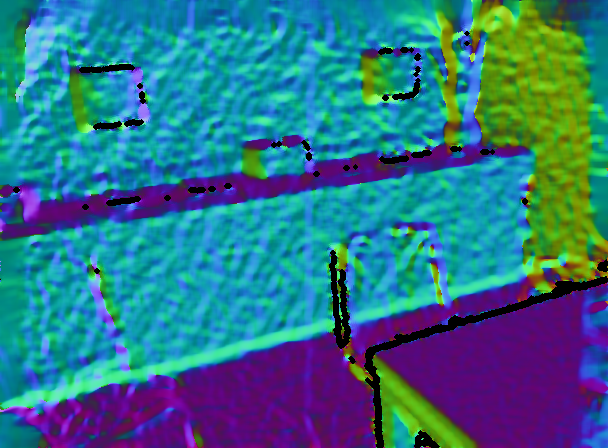
\includegraphics[scale=\scalefivenyu]{pictures/nyu-1-normals-color}
	}
	\subfigure{
		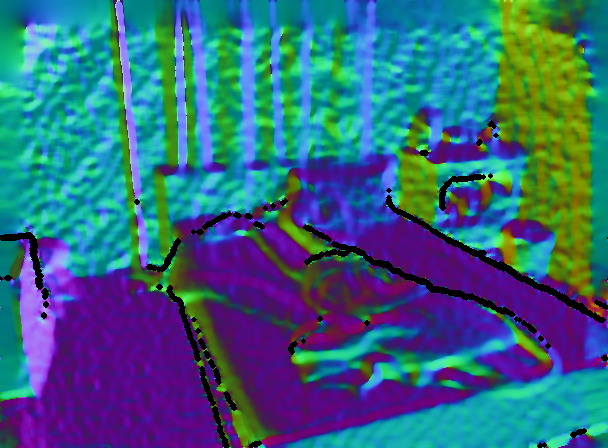
\includegraphics[scale=\scalefivenyu]{pictures/nyu-2-normals-color}
	}
	\subfigure{
		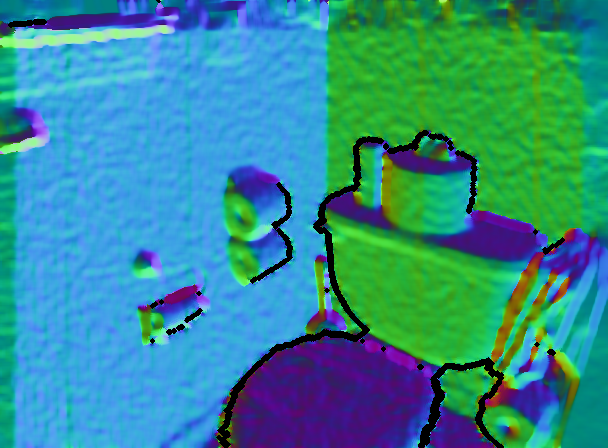
\includegraphics[scale=\scalefivenyu]{pictures/nyu-3-normals-color}
	}
	\subfigure{
		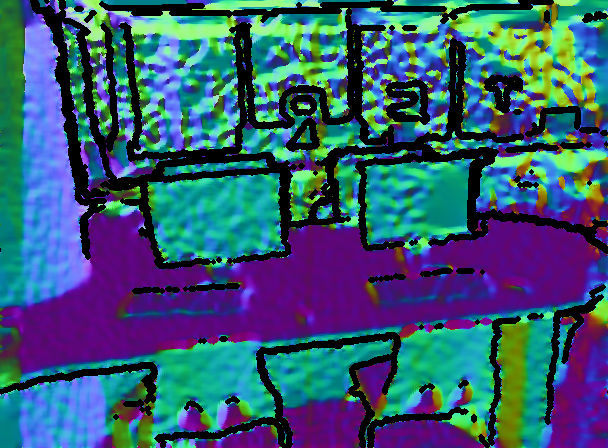
\includegraphics[scale=\scalefivenyu]{pictures/nyu-4-normals-color}
	}
	\subfigure{
		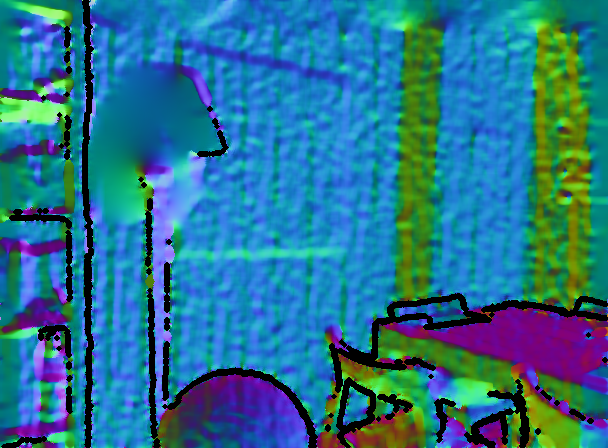
\includegraphics[scale=\scalefivenyu]{pictures/nyu-5-normals-color}
	}
	\subfigure{
		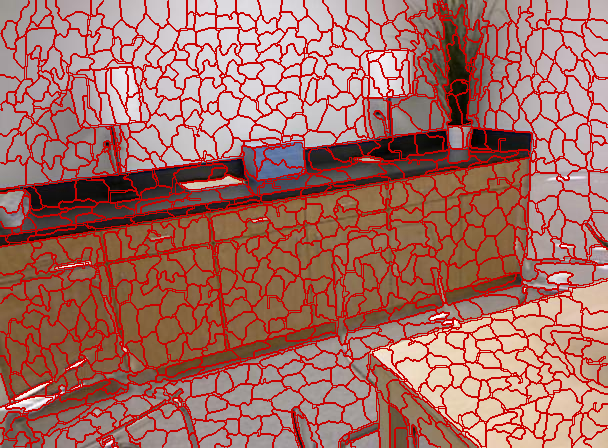
\includegraphics[scale=\scalefivenyu]{pictures/nyu-1-seeds3dn}
	}
	\subfigure{
		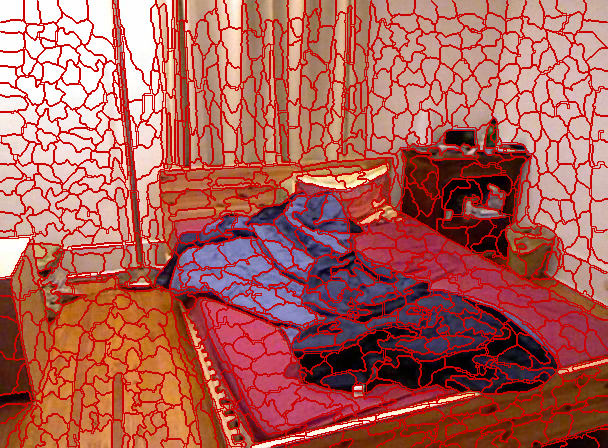
\includegraphics[scale=\scalefivenyu]{pictures/nyu-2-seeds3dn}
	}
	\subfigure{
		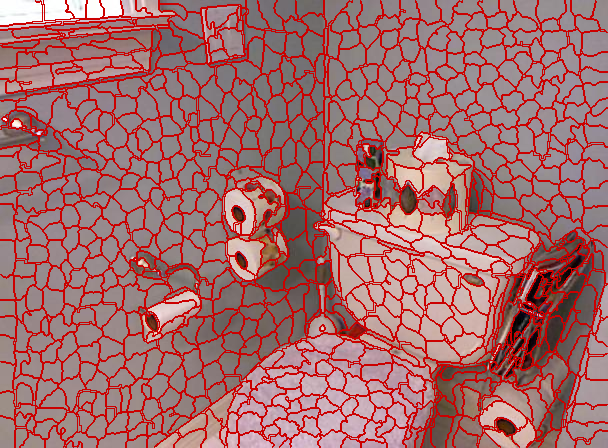
\includegraphics[scale=\scalefivenyu]{pictures/nyu-3-seeds3dn}
	}
	\subfigure{
		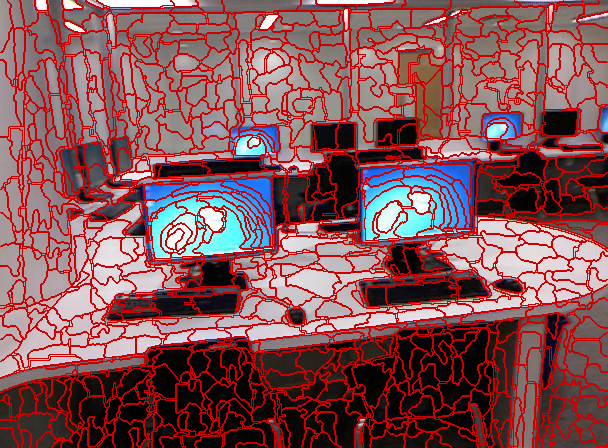
\includegraphics[scale=\scalefivenyu]{pictures/nyu-4-seeds3dn}
	}
	\subfigure{
		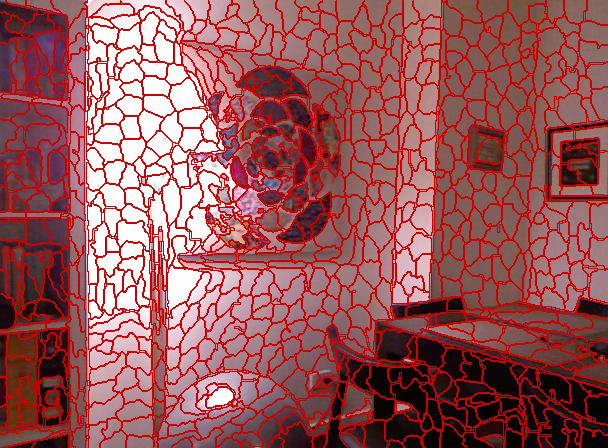
\includegraphics[scale=\scalefivenyu]{pictures/nyu-5-seeds3dn}
	}
	\caption[Estimated normals of the running examples color coded and superpixel segmentations generated by an extension of \textbf{SEEDS} \cite{VanDenBerghBoixRoigCapitaniVanGool:2012} using normal information.]{Top: estimated normals for the running examples color coded -- black indicates that no normal could be estimated for this particular pixel. Bottom: the running examples oversegmented into exactly $840$ superpixels using \textbf{SEEDS3Dn}.}
	\label{fig:seeds-depth-3d-normal-mean-pixels-normal-computation}
\end{figure}

As experiments in chapter \ref{chapter:evaluation} show, using normal information for pixel updates results in a negligible performance increase when the normal information is weighted sufficiently low. Whether this is due to the noisy normal computation or the fact that superpixel algorithms using color and 3D point coordinates only already perform well needs to be verified on different datasets. Overall, the running examples oversegmented using \textbf{SEEDS3Dn} are shown in figure \ref{fig:seeds-depth-3d-normal-mean-pixels-normal-computation}.

\section{Mean-Based Block Updates}
\label{section:seeds-depth-mean-block-updates}

Color histograms offer a suitable representation for blocks of pixels. However, as approaches like \textbf{SLIC} \cite{AchantaShajiSmithLucchiFuaSuesstrunk:2010}, \textbf{DASP} and \textbf{VCCS} successfully apply the concept of superpixel centers to superpixel segmentation, it may be beneficial to use similar representations for block updates as well. Consequently, each block $B_i^{(l)}$ is represented by its center and its similarity to a superpixel $S_j$ can be expressed as distance:
\begin{align}
	\label{eq:seeds-depth-mean-block-updates-distance}
	d(B_i^{(l)}, S_j) = \|I(B_i^{(l)}) - I(S_j)\|_2 + \beta\|P(B_i^{(l)}) - P(S_j)\|_2.
\end{align}
The block centers can be pre-computed during initialization, see algorithm \ref{algo:seeds-depth-mean-block-updates}.

The above concept can also be extended to use normal information. In practice, this amounts to computing the blocks mean color and position as well as its orientation. In the simplest form, the orientation $N(B_i^{(l)})$ of block $B_i^{(l)}$ is given by the average of the orientations $N(x_n)$ of the corresponding pixels such that the similarity of block $B_i^{(l)}$ and superpixel $S_j$ can be expressed as
\begin{align}
	d(B_i^{(l)}, S_j) = &\|I(B_i^{(l)}) - I(S_j)\|_2 + \beta\|P(B_i^{(l)}) - P(S_j)\|_2\notag\\
	& + \gamma \arccos \left(N(B_i^{(l)})^T N(S_j) \right).
\end{align}
This is the natural extension of \textbf{SEEDS3Dn} to block updates. Together, the position $P(B_i^{(l)})$ and the orientation $N(B_i^{(l)})$ can be interpreted as plane such that the orientation could also be estimated using a plane fit.
\begin{algorithm}[t]
	\begin{algo}{SEEDS (mean block updates)}{\label{algo:seeds-depth-mean-block-updates}\qinput{color image $I$, block size $w^{(1)} \times h^{(1)}$, number of levels $L$}\qoutput{superpixel segmentation $S$}}
		initialize the block hierarchy and the initial superpixel segmentation $S$\\
		\qcom{Initialization of block/superpixel centers:}\\
		\qfor $l = 1$ \qto $L$\\
			\qforeach block $B_i^{(l)}$ at level $l$ \qcom{For $l = L$ these are the initial superpixels.}\\ 
				compute $I(B_i^{(l)})$ and $P(B_i^{(l)})$\qrof\qrof\\
		\qcom{Mean based block updates:}\\
		\qfor $l = L - 1$ \qto $1$\\
			\qforeach block $B_i^{(l)}$ at level $l$\\
				let $S_j$ be the superpixel $B_i^{(l)}$ belongs to\\
				\qif a neighboring block belongs to a different superpixel $S_k$\\
					\qthen \qif $d(B_i^{(l)}, S_k) < d(B_i^{(l)}, S_j)$\\
						\qthen $S_k$ \qlet $S_k \cup B_i^{(l)}$ and $S_j$ \qlet $S_j - B_i^{(l)}$\qfi\qfi\qrof\qrof\\
		%\qcom{Note that for mean pixel updates, the superpixel centers are already computed.}\\
		mean pixel updates \qcom{Note that the superpixel centers are already available.}\\
		\qreturn S
	\end{algo}
	\caption[\textbf{SEEDS} \cite{VanDenBerghBoixRoigCapitaniVanGool:2012} based on mean block updates using 3D point coordinates.]{After defining a distance $d(B_i^{(l)}, S_j)$ between blocks and superpixels based on their respective centers, block updates can be performed without relying on color histograms. Of course, both approaches can also be combined resulting in a higher runtime}
	\label{fig:seeds-depth-mean-block-updates}
\end{algorithm}

\subsection{Discussion}

Unfortunately, block centers appear to be a poor representation for blocks of pixels. For example consider the running examples in figure \ref{fig:seeds-depth-mean-block-updates-discussion-blocks}. Choosing a block crossing a strong boundary between different objects, a color histogram is able to capture both parts of the block by having two modes. However, the block center may capture information not present within the block. In contrast, superpixels computed after performing block updates at level $l = 1$ appear to be homogeneous in color and cover mostly one object such that using superpixel centers is appropriate for pixel updates. Therefore, using mean position and color as representation of superpixels is appropriate only when given a sound initial superpixel segmentation and consequently blocks of pixels are better represented by color histograms.
\begin{figure}[t]
	\centering
	\subfigure{
		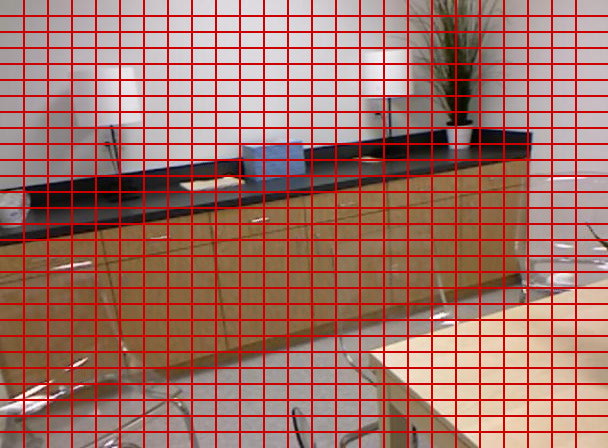
\includegraphics[scale=\scalefivenyu]{pictures/nyu-1-seeds-level-4}
	}
	\subfigure{
		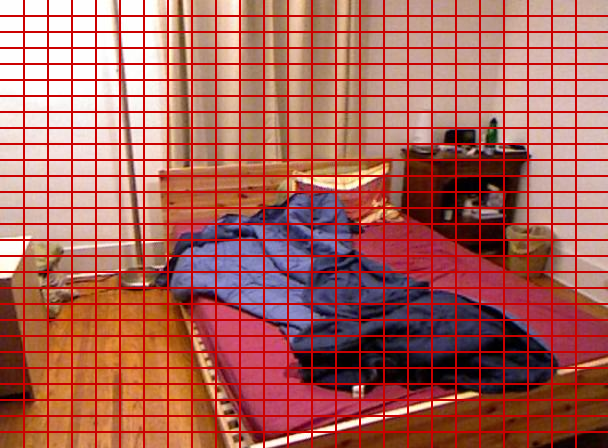
\includegraphics[scale=\scalefivenyu]{pictures/nyu-2-seeds-level-4}
	}
	\subfigure{
		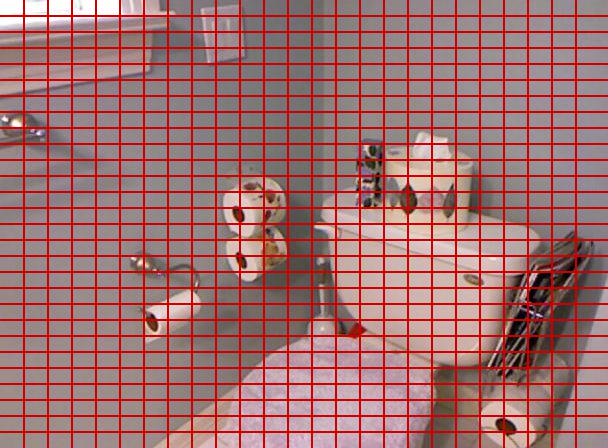
\includegraphics[scale=\scalefivenyu]{pictures/nyu-3-seeds-level-4}
	}
	\subfigure{
		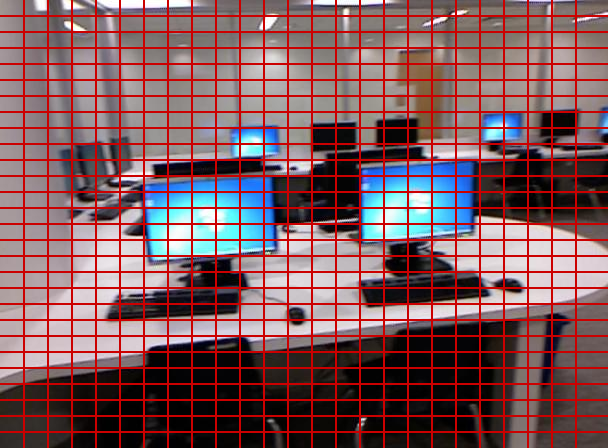
\includegraphics[scale=\scalefivenyu]{pictures/nyu-4-seeds-level-4}
	}
	\subfigure{
		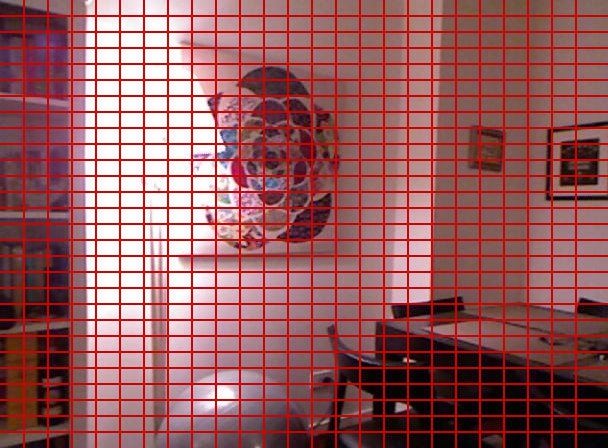
\includegraphics[scale=\scalefivenyu]{pictures/nyu-5-seeds-level-4}
	}
	\subfigure{
		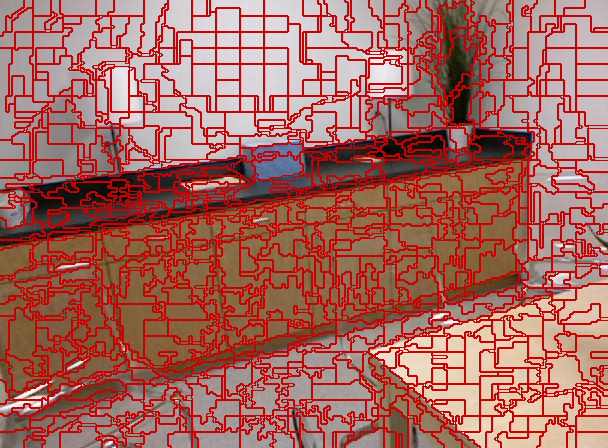
\includegraphics[scale=\scalefivenyu]{pictures/nyu-1-seeds-after-1}
	}
	\subfigure{
		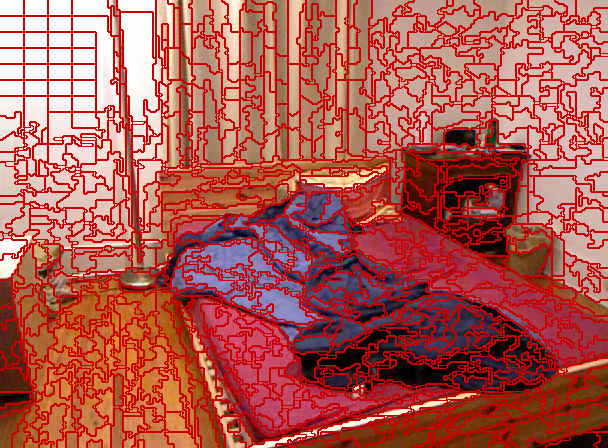
\includegraphics[scale=\scalefivenyu]{pictures/nyu-2-seeds-after-1}
	}
	\subfigure{
		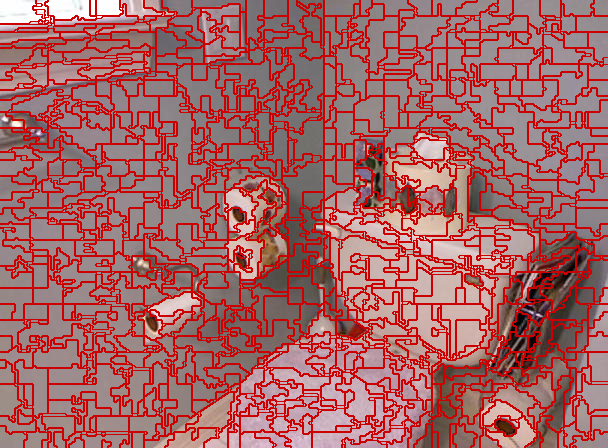
\includegraphics[scale=\scalefivenyu]{pictures/nyu-3-seeds-after-1}
	}
	\subfigure{
		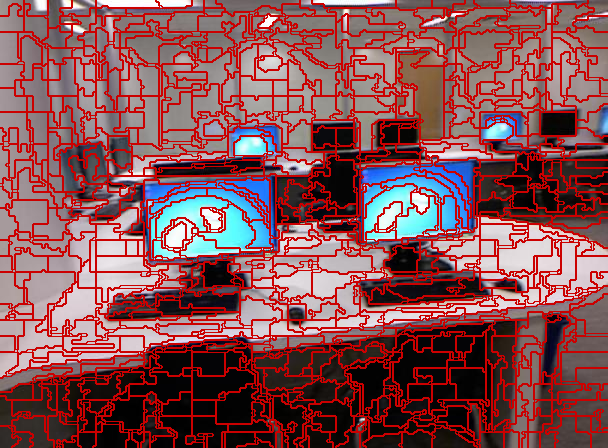
\includegraphics[scale=\scalefivenyu]{pictures/nyu-4-seeds-after-1}
	}
	\subfigure{
		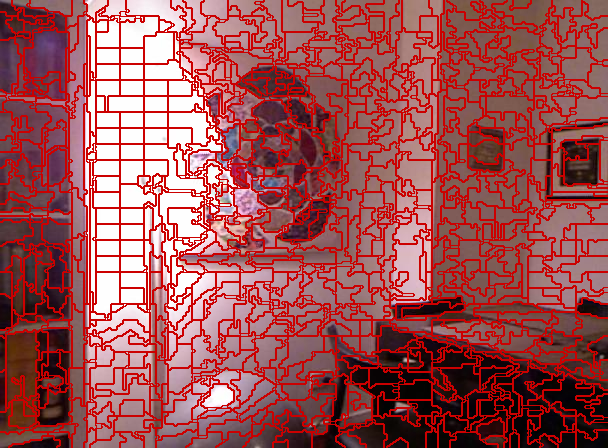
\includegraphics[scale=\scalefivenyu]{pictures/nyu-5-seeds-after-1}
	}
	\caption[An illustration of the disadvantages of using block centers to perform block updates.]{Top: Block segmentations at level $(L - 1)$. Bottom: superpixel segmentations before performing pixel updates.}
	\label{fig:seeds-depth-mean-block-updates-discussion-blocks}
\end{figure}
The same considerations apply for averaging normals. Therefore, we used the covariance matrix to estimate the orientation of the blocks and superpixels. However, after each update, the orientation of the corresponding superpixels need to be recomputed. Although this approach is comparably inefficient, our experiments show that even after computing the optimal orientation in the least squares sense, using normal information does not increase performance.
Furthermore, computing block centers at lower levels, where each block contains only few pixels, is highly influenced by outliers and noise. Overall, these considerations imply that mean based block updates perform poorly when compared to the original block updates in algorithm \ref{algo:superpixel-segmentation-seeds}. This can also be interpreted as motivation of superpixel growing as done by \textbf{SLIC}, \textbf{DASP} and \textbf{VCCS}.

% TODO: Introduce "3D mean pixels".
%The above discussion can be supported by experiments. Figure \ref{fig:seeds-depth-mean-block-updates-discussion-comparison} compares several images when segmented using usual block updates and 3D mean pixel updates and mean based block updates.
%\begin{figure}
%	% TODO: runnign examples compared (have to reimplement mean based updates).
%	\label{fig:seeds-depth-mean-block-updates-discussion-comparison}
%\end{figure}

\section{Block Updates Based on Normal Histograms}
\label{section:deeds-depth-normal-histograms}

As color histograms appear to work well as representations for blocks of pixels, it appears to be advantageous to integrate depth information in the form of histograms. Depth histograms, however, do not offer an increase in performance. Therefore, we would like block updates to capture normal information instead. This can be accomplished using histograms of normal orientation which we refer to as normal histograms.

Given a point normal $N(x_n)$ with components $N_1(x_n), N_2(x_n), N_3(x_n)$, the orientation can be split up into the polar angle $\phi$ between normal and the y-axis, and the azimuthal angle $\theta$ between normal and x-axis, see figure \ref{fig:seeds-depth-normal-histograms-angles}.
The angles are binned to form a two dimensional histogram and the similarity of a block and a superpixel is then expressed as the intersection of these histograms. This can be weighted and used in combination with color histograms.
% taken from: http://www.texample.net/tikz/examples/the-3dplot-package/
\begin{SCfigure}[2\sidecaptionrelwidth][b]
	%set the plot display orientation
	%synatax: \tdplotsetdisplay{\theta_d}{\phi_d}
	\tdplotsetmaincoords{60}{110}

	%define polar coordinates for some vector
	%TODO: look into using 3d spherical coordinate system
	\pgfmathsetmacro{\rvec}{.4}
	\pgfmathsetmacro{\thetavec}{30}
	\pgfmathsetmacro{\phivec}{60}
	\begin{tikzpicture}[scale=5,tdplot_main_coords]

		%set up some coordinates 
		%-----------------------
		\coordinate (O) at (0,0,0);
		
		%determine a coordinate (P) using (r,\theta,\phi) coordinates.  This command
		%also determines (Pxy), (Pxz), and (Pyz): the xy-, xz-, and yz-projections
		%of the point (P).
		%syntax: \tdplotsetcoord{Coordinate name without parentheses}{r}{\theta}{\phi}
		\tdplotsetcoord{P}{\rvec}{\thetavec}{\phivec}
		\tdplotsetcoord{N}{\rvec + 0.2}{\thetavec}{\phivec}

		%draw figure contents
		%--------------------

		%draw the main coordinate system axes
		\draw[thick,->] (0,0,0) -- (0.5,0,0) node[anchor=north east]{$x$};
		\draw[thick,->] (0,0,0) -- (0,0.5,0) node[anchor=north west]{$z$};
		\draw[thick,->] (0,0,0) -- (0,0,0.5) node[anchor=south]{$y$};
		
		%draw a vector from origin to point (P) 
		\draw[-stealth,color=red] (O) -- (P);
		\node at (N) {$N(x_n)$};

		%draw projection on xy plane, and a connecting line
		\draw[dashed, color=red] (O) -- (Pxy);
		\draw[dashed, color=red] (P) -- (Pxy);

		%draw the angle \phi, and label it
		%syntax: \tdplotdrawarc[coordinate frame, draw options]{center point}{r}{angle}{label options}{label}
		\tdplotdrawarc{(O)}{0.15}{0}{\phivec}{anchor=north}{$\theta$}

		%set the rotated coordinate system so the x'-y' plane lies within the
		%"theta plane" of the main coordinate system
		%syntax: \tdplotsetthetaplanecoords{\phi}
		\tdplotsetthetaplanecoords{\phivec}

		%draw theta arc and label, using rotated coordinate system
		\tdplotdrawarc[tdplot_rotated_coords]{(0,0,0)}{0.25}{0}{\thetavec}{anchor=south}{$\phi$}

		%draw some dashed arcs, demonstrating direct arc drawing
		\draw[dashed,tdplot_rotated_coords] (\rvec,0,0) arc (0:90:\rvec);
		\draw[dashed] (\rvec,0,0) arc (0:90:\rvec);

		%set the rotated coordinate definition within display using a translation
		%coordinate and Euler angles in the "z(\alpha)y(\beta)z(\gamma)" euler rotation convention
		%syntax: \tdplotsetrotatedcoords{\alpha}{\beta}{\gamma}
		\tdplotsetrotatedcoords{\phivec}{\thetavec}{0}

		%translate the rotated coordinate system
		%syntax: \tdplotsetrotatedcoordsorigin{point}
		\tdplotsetrotatedcoordsorigin{(P)}

		%change the rotated coordinate frame so that it lies in its theta plane.
		%Note that this overwrites the original rotated coordinate frame
		%syntax: \tdplotsetrotatedthetaplanecoords{\phi'}
		\tdplotsetrotatedthetaplanecoords{45}

	\end{tikzpicture}
	\caption[Illustration of the binning of normal orientation into histograms.]{Point normals are binned using the polar angle $\phi$ between normal and $y$-axis and the azimuthal angle $\theta$ between normal and $x$-axis. In practice, the normal is always oriented towards the viewpoint such that $\phi, \theta \in [0,180^\circ]$.}
	\label{fig:seeds-depth-normal-histograms-angles}
\end{SCfigure}

\subsection{Discussion}
\label{subsection:deeds-depth-normal-histograms-discussion}

Considering the binning of the normals, we came to the conclusion that an odd number of bins per angle should be used. This is based on the following case: We consider a normal with $\phi = 90^\circ$ and $\theta = 90^\circ$. As this normal is not estimated perfectly, the angles would lie slightly below or above the $90^\circ$ such that the actual bin depends on the noise and the estimation method which should be avoided to get an adequate representation of surfaces parallel to the image plane.
%This is illustrated in figure \ref{fig:seeds-depth-normal-histograms-binning}.
%\begin{figure}
%	% TODO: figure for binning.
%	\label{fig:seeds-depth-normal-histograms-binning}
%\end{figure}

Overall, experiments show that this extension does not improve performance while additionally increasing runtime. In our opinion, the main reasons for this observation are the following. Firstly, as stated in section \ref{section:seeds-depth-3d-normal-mean-pixel-updates}, a superpixel segmentation obtained by running \textbf{SEEDS} based purely on color achieves state-of-the-art performance leaving only little room for improvement. Secondly, the most difficult regions within images taken from the NYU Depth Dataset \cite{SilbermanHoiemKohliFergus:2012} contain plenty of small objects -- often the scenes are highly cluttered. In such settings, the estimated normals tend to be highly unrepresentative and noisy. In contrast, in regions of nearly planar surfaces, where we expect normal information to be of help, oversegmentations based on color only usually yield high performance. In conclusion, we find that normal histograms are not worth their computation time. Figure \ref{fig:seeds-depth-normal-histograms-comparison} shows the running examples oversegmented using normal histograms. As pixel updates have not been adapted, the results differ only slightly from those presented in figure \ref{fig:seeds-depth-3d-mean-pixels-comparison}. In contrast, when using pixel updates based on color and normal histograms similar to those in algorithm \ref{algo:superpixel-segmentation-seeds}, the superpixel segmentations appear to have low quality.
\begin{figure}[t]
	\centering
	\subfigure{
		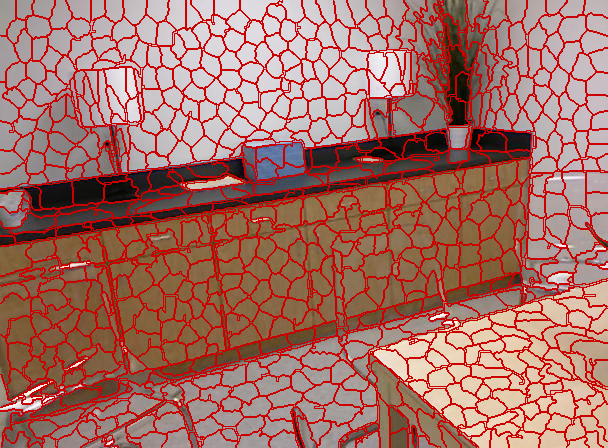
\includegraphics[scale=\scalefivenyu]{pictures/nyu-1-seeds-normal-histograms}
	}
	\subfigure{
		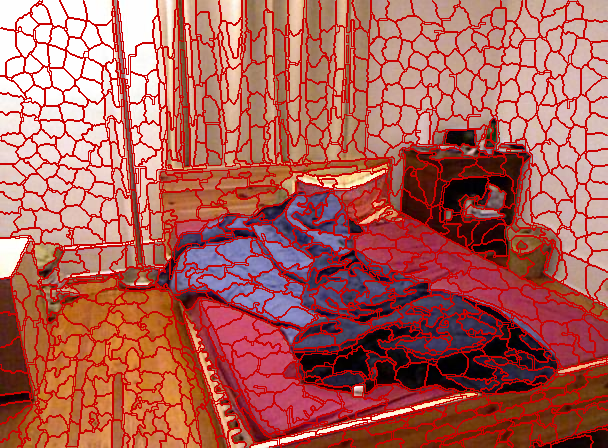
\includegraphics[scale=\scalefivenyu]{pictures/nyu-2-seeds-normal-histograms}
	}
	\subfigure{
		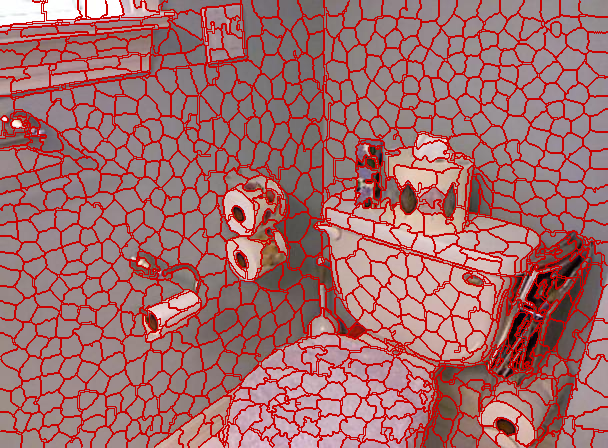
\includegraphics[scale=\scalefivenyu]{pictures/nyu-3-seeds-normal-histograms}
	}
	\subfigure{
		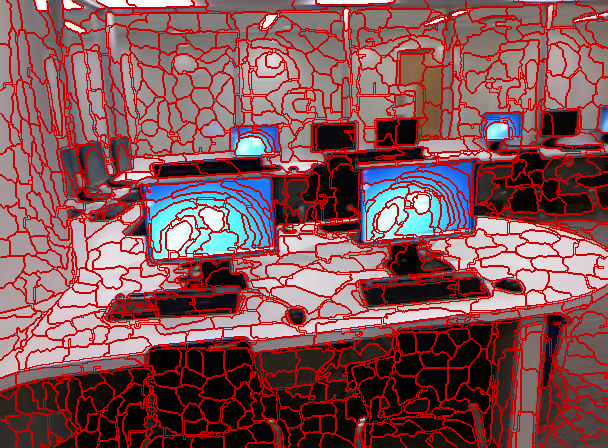
\includegraphics[scale=\scalefivenyu]{pictures/nyu-4-seeds-normal-histograms}
	}
	\subfigure{
		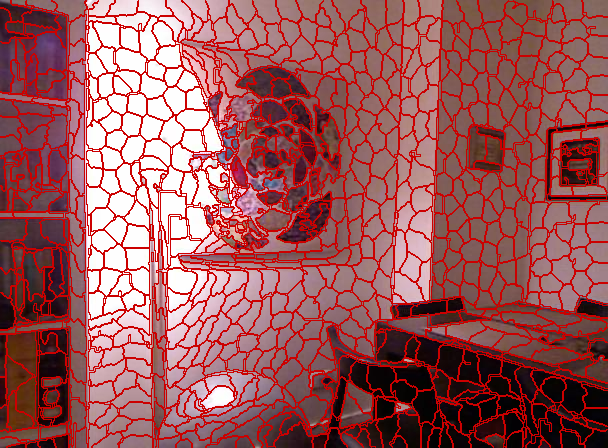
\includegraphics[scale=\scalefivenyu]{pictures/nyu-5-seeds-normal-histograms}
	}
	\subfigure{
		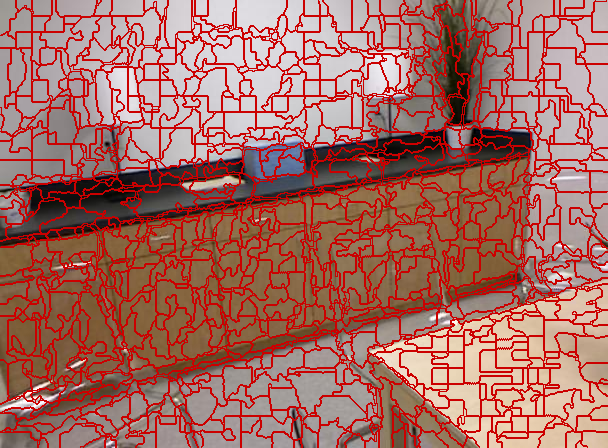
\includegraphics[scale=\scalefivenyu]{pictures/nyu-1-seeds-normal-histograms-pixel}
	}
	\subfigure{
		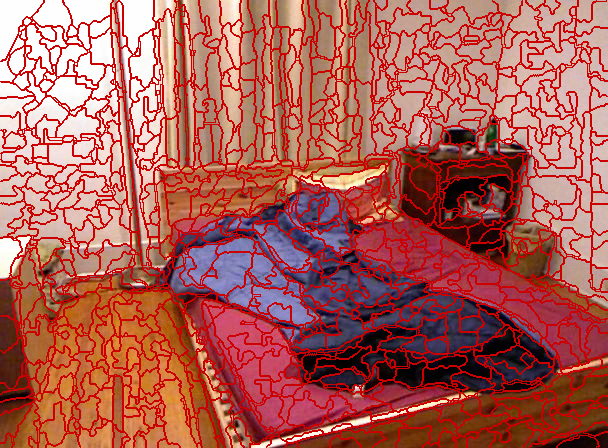
\includegraphics[scale=\scalefivenyu]{pictures/nyu-2-seeds-normal-histograms-pixel}
	}
	\subfigure{
		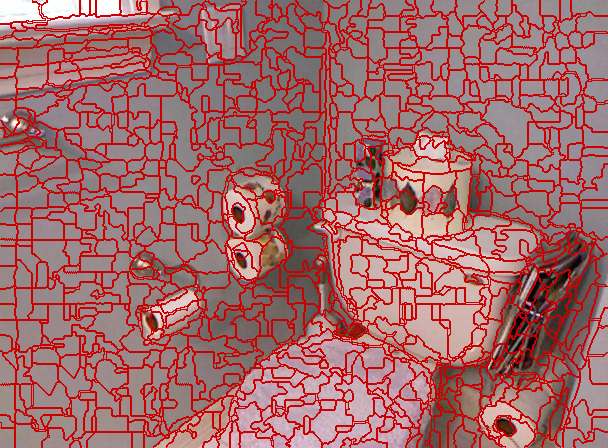
\includegraphics[scale=\scalefivenyu]{pictures/nyu-3-seeds-normal-histograms-pixel}
	}
	\subfigure{
		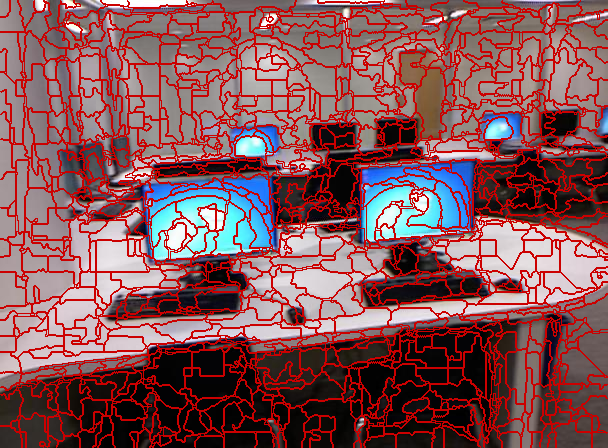
\includegraphics[scale=\scalefivenyu]{pictures/nyu-4-seeds-normal-histograms-pixel}
	}
	\subfigure{
		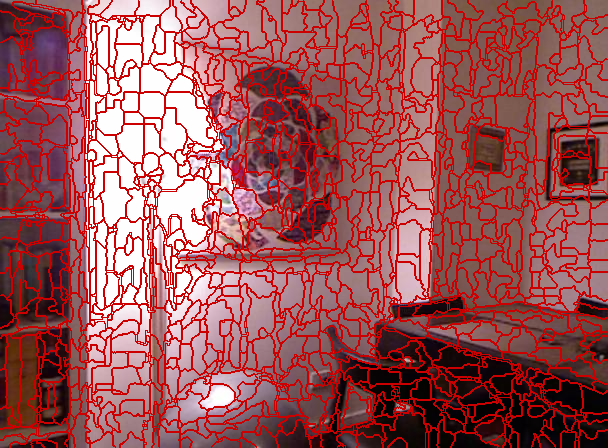
\includegraphics[scale=\scalefivenyu]{pictures/nyu-5-seeds-normal-histograms-pixel}
	}
	\caption[Superpixel segmentations of the running examples generated by a variant of \textbf{SEEDS} \cite{VanDenBerghBoixRoigCapitaniVanGool:2012} based on normal histograms.]{Top: the running examples oversegmented using normal histograms for block updates. Bottom: superpixel segmentations with exactly $840$ superpixels of the running examples generated using normal histograms for both block updates and pixel updates.}
	\label{fig:seeds-depth-normal-histograms-comparison}
\end{figure}

%\section{Block Updates Based on Plane Fitting}
%
%Combining both normal information as well as the concept of block centers, an interesting representation of a block of pixels is given by a plane fit for the corresponding 3D point coordinates. Similar to normal estimation, this can be done using the covariance matrix of all points $P(x_n)$ within the block. However, the covariance matrix of each superpixel has to be recomputed after each block or pixel update based on the superpixel's center. An alternative is given by averaging methods as for example described by Klasing \etal \cite{KlasingAlthoffWollherrBuss:2009}. Using averaging methods, planes could be estimated incrementally such that block and pixel updates can be performed more efficiently. In its simplest form this would mean to average the point normals $N(x_n)$ for all points within the block. Overall, given a block $B_i^{(l)}$ and a superpixel $S_j$, we can compute the angle between the corresponding normals to get a further clue of their similarity:
%\begin{align}
%	\arccos\left(N(B_i^{(l)})^T N(S_j)\right).
%\end{align}
%This can 
%
%In the following, we review the above considerations in detail.\\
%Plane Fitting: Given a block $B_i^{(l)}$ with pixels $x_{n_1},\ldots,x_{n_k}$, we aim to fit a plane characterized by
%\begin{align}
%	\label{eq:seeds-depth-plane}
%	N_1(B_i^{(l)}) P_1(x_{n_j}) + N_3(B_i^{(l)}) P_3(x_{n_j}) + N_3(B_i^{(l)}) P_3(x_{n_j}) + d = 0\quad \forall 1 \leq j \leq k.
%\end{align}
%This leads to solving
%\begin{align}
%	\left\| \begin{pmatrix} \boldsymbol P &\boldsymbol 1 \end{pmatrix} \begin{pmatrix} N_1(B_i^{(l)})\\ N_2(B_i^{(l)})\\ N_3(B_i^{(l)}) \end{pmatrix} \right\|_2 \rightarrow \min
%\end{align}
%where $\boldsymbol P$ is the matrix containing the points $P(x_{n_1}), \ldots, P(x_{n_k})$ in its rows and $\boldsymbol 1~=~(1, \ldots, 1)^T$. This can be solved utilizing Singular Value Decomposition (\eg see \cite{ForsythPonce:2002}).\\
%%As alternative, the mean can be computed as usual and the normal can be estimated using an averaging method. Let $T(B_i^{(l)})$ be the set of all subsets of size three of $B_i^{(l)}$. Then the normal can be estimated as
%%\begin{align}
%%	N(B_i^{(l)}) = \frac{1}{|T(B_i^{(l)})|} \sum_{\{x_i,x_j,x_k\} \in T(b_i^{(l)})  \frac{(x_j - x_i) \times (x_k - x_i)}{\|(x_j - x_i) \times (x_k - x_i)\|_2}
%%\end{align}
%%where $\times$ denotes the cross product. The uniform weighting factor can also be replaced by their weighting schemes \cite{KlasingAlthoffWollherrBuss:2009}. Such an estimate can be updated easily after exchanging blocks or pixels.
%% TODO: check correct angle comptuation for DASP, VCCS, 3D (Normal) Mean Pixels
%Block Updates: Given block $B_i^{(l)}$ and superpixel $S_j$, the similarity of block $B_i^{(l)}$ to superpixel $S_j$ can be expressed as
%\begin{align}
%	d(B_i^{(l)}, S_j) = \frac{N(B_i^{(l)})^T N(S_j)}{\|N(B_i^{(l)})\|_2 \|N(S_j)\|_2}.
%\end{align}
%This can then be combined with color histograms and is similar to using mean block updates where additionally normal information is used to characterize the block and superpixel centers.\\
%Pixel Updates: The distance of a point $P(x_n)$ to the plane of superpixel $S_j$ can be calculated as
%\begin{align}
%	d(x_n, S_j) = \frac{(P(x_n) - P(S_j))^T N(S_j)}{\|N(S_j)\|_2}.
%\end{align}
%However, the euclidean distance to the superpixel center appears to be more appropriate and reliable as the above equation performs an orthogonal projection. Again, this has to be combined with a color term which is either based on color histograms or the euclidean distance in color space.\\
%Overall, the above considerations are similar to the idea of performing mean based block updates. When using averaging methods to estimate the plane of equation \eqref{eq:seeds-depth-plane} this approach actually boils down to use mean based block updates with normal information. However, estimating the planes based on sufficient statistics which could be updated incremental is possible as well.
%
%\subsection{Discussion}
%
%As discussed in sections \ref{section:seeds-depth-mean-block-updates} and \ref{section:seeds-depth-3d-normal-mean-pixel-updates}, the main problem with this approach is the initial superpixel segmentation. The fitted planes are initially highly unrepresentative. For small blocks, noisy pixels and outliers worsen the estimated planes. Furthermore, the most interesting and difficult objects within the scenes cannot be represented by a set of planes (see discussion in section \ref{subsection:deeds-depth-normal-histograms-discussion}). Overall, as we expected after experimenting with normal histograms, planes are not an appropriate representation and strongly increase runtime as well as performance.